\RequirePackage{tikz}

\usepackage{avant} % A font similar to Century Gothic
\usepackage{courier} % Courier font for code listings
\usepackage{graphicx}
\usepackage{listings}
\lstset{
	basicstyle=\footnotesize\ttfamily,
	frame=single,
	tabsize=4,
	showstringspaces=false,
	breaklines=true,
	prebreak={\space\hbox{\textcolor{Gray}{$\hookleftarrow$}}}
}

\graphicspath{ {FalmouthGamesAcademyTheme/} }

\hypersetup{
    colorlinks=true,
    linkcolor=white,
    filecolor=magenta,      
    urlcolor=cyan,
}


\iftoggle{printable}{
	\lstset{
		commentstyle=\ttfamily\textit,
		keywordstyle=\ttfamily\textbf,
		stringstyle=\ttfamily,
		rulecolor=\color{Black}
	}
}{ % else
	\lstset{
		commentstyle=\color{LimeGreen}\ttfamily\textit,
		keywordstyle=\color{SkyBlue}\ttfamily\textbf,
		stringstyle=\color{Melon}\ttfamily,
		rulecolor=\color{White}
	}
}

%\setbeamercovered{transparent}

\definecolor{GamesAcademyPurple}{rgb}{0.25,0.19,0.32}
\definecolor{SubtitleGrey}{rgb}{0.53,0.53,0.53}

\iftoggle{printable}{
	\usecolortheme{default}
	\setbeamercolor{normal text}{fg=black,bg=white}
	\setbeamercolor{frametitle}{fg=black}
	\setbeamercolor{itemize item}{fg=black}
	\setbeamercolor{enumerate item}{fg=black}
	\setbeamercolor{subtitle}{fg=black}
}{ % else
	\usecolortheme{albatross}
	\setbeamercolor{normal text}{fg=white,bg=GamesAcademyPurple}
	\setbeamercolor{frametitle}{fg=white}
	\setbeamercolor{itemize item}{fg=white}
	\setbeamercolor{enumerate item}{fg=white}
	\setbeamercolor{subtitle}{fg=SubtitleGrey}
}

\newlength{\PptPoint}
\setlength{\PptPoint}{0.5pt}
\setbeamerfont{title}{size=\fontsize{40\PptPoint}{40\PptPoint}}
\setbeamerfont{subtitle}{size=\fontsize{24\PptPoint}{24\PptPoint}}
\setbeamerfont{frametitle}{size=\fontsize{40\PptPoint}{40\PptPoint}}

\setbeamertemplate{title page}{
    \begin{tikzpicture}[remember picture,overlay]
    	\iftoggle{printable}{}{
			\node[anchor=north, xshift=0cm, yshift=0.12cm] (banner) at (current page.north) {
				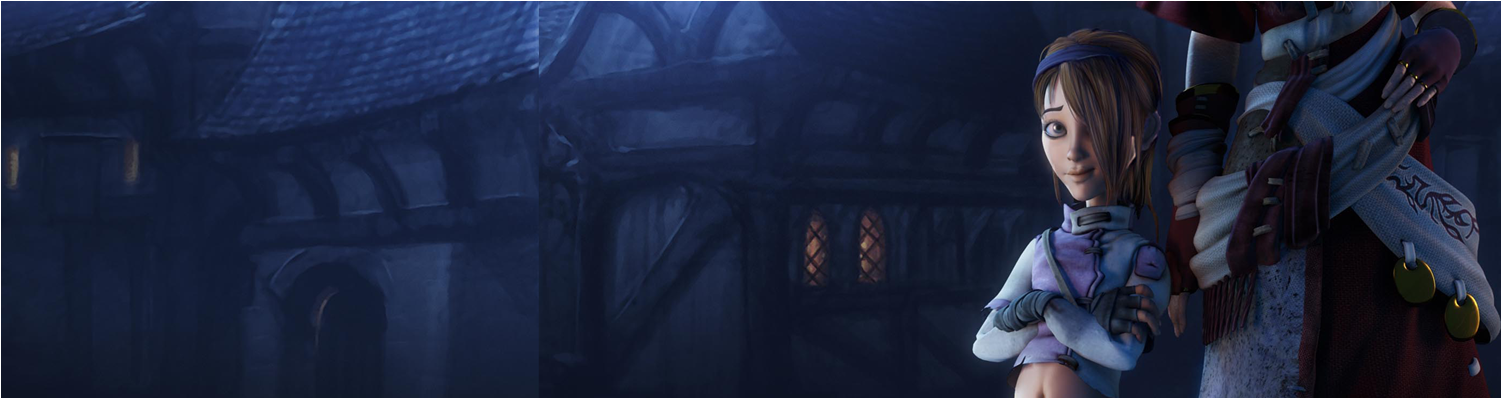
\includegraphics[width=\paperwidth]{template_girl}
			};
			\node[anchor=south west, xshift=0.1cm, yshift=0.1cm] at (banner.south west) {
				
\includegraphics[width=0.1\paperwidth]{template_falmouth_logo}
			};
		}
        \node(Title)[anchor=south east, xshift=-0.025\paperwidth, yshift=40\PptPoint] at (current page.south east) {
			\parbox[t]{0.95\paperwidth}{\raggedleft\usebeamerfont{title}\textbf{\inserttitle}}
        };
        \node[anchor=south east, yshift=-0.1cm] at (Title.north east) {
        	\parbox[t]{0.95\paperwidth}{\raggedleft\usebeamerfont{subtitle}\textcolor{SubtitleGrey}{\insertsubtitle}}
        };
    \end{tikzpicture}
}

\setbeamertemplate{headline}{
    \begin{tikzpicture}[remember picture,overlay]
    	\iftoggle{printable}{}{
			\node[anchor=north, xshift=0cm, yshift=0.12cm] (head) at (current page.north) {
				
\includegraphics[width=\paperwidth]{template_head}
			};
			\node[anchor=north west, xshift=0.1cm, yshift=-0.1cm] at (current page.north west) {
				
\includegraphics[width=0.1\paperwidth]{template_falmouth_logo}
			};
		}
    \end{tikzpicture}
    \vspace*{0.7cm}
}

\setbeamertemplate{frametitle}[default][center]

\setbeamertemplate{part page}{
    \begin{tikzpicture}[remember picture,overlay]
    	\iftoggle{printable}{}{
			\fill [GamesAcademyPurple] (current page.north west) rectangle (current page.south east);
			\node[anchor=north west, xshift=0.1cm, yshift=-0.1cm] at (current page.north west) {
				
\includegraphics[width=0.1\paperwidth]{template_falmouth_logo}
			};
			\node[anchor=south east, xshift=0.2cm, yshift=0.2cm] at (current page.south east) {
				
\includegraphics[height=\paperheight]{template_man}
			};
		}
        \node[anchor=south west, xshift=0.05\paperwidth, yshift=80\PptPoint] at (current page.south west) {
			\parbox[t]{0.9\paperwidth}{\raggedright\usebeamerfont{title}\textbf{\insertpart}}
        };
    \end{tikzpicture}
}
